\documentclass[11pt,a4paper]{article}

% Configuración de página y márgenes
\usepackage[margin=1in, top=1.2in, bottom=1.2in]{geometry}

% Paquetes para caracteres especiales y codificación
\usepackage[utf8]{inputenc}
\usepackage[T1]{fontenc}
\usepackage{lmodern}

% Soporte para idiomas (español e inglés)
\usepackage[spanish,english]{babel}

% Paquetes para imágenes y gráficos
\usepackage{graphicx}
\usepackage{float}
\usepackage{caption}
\usepackage{subcaption}

% Paquetes para tablas
\usepackage{longtable}
\usepackage{booktabs}
\usepackage{array}
\usepackage{multirow}
\usepackage{multicol}
\usepackage{tabularx}

% Control de saltos de página
\usepackage{needspace}
\usepackage{afterpage}
\usepackage{placeins}

% Enlaces e hipervínculos
\usepackage[colorlinks=true, linkcolor=blue, urlcolor=blue, citecolor=blue]{hyperref}

% Paquetes para código y verbatim
\usepackage{fancyvrb}
\usepackage{listings}
\usepackage{xcolor}

% Configuración de listings para código
\lstset{
    basicstyle=\ttfamily\small,
    breaklines=true,
    frame=single,
    backgroundcolor=\color{gray!10},
    keywordstyle=\color{blue},
    commentstyle=\color{green!50!black},
    stringstyle=\color{red}
}

% Paquetes para mejor tipografía
\usepackage{microtype}
\usepackage{setspace}

% Configuración de espaciado
\onehalfspacing

% Comandos personalizados
\providecommand{\tightlist}{}

% Comando para evitar viudas y huérfanas
\widowpenalty=10000
\clubpenalty=10000

% Configuración de profundidad de numeración
\setcounter{secnumdepth}{3}
\setcounter{tocdepth}{3}

\begin{document}


    
    % Título principal
    {\Huge \textbf{DevLab Module Datasheet}}\\[1.5em]
    
    % Subtítulo si existe
    
    
    % Autor
    
    
    % Fecha
    
    
    \vfill
    
    % Información adicional al pie
    
    
    
\end{titlepage}

% Tabla de contenidos


% Lista de figuras (si hay imágenes)


% Lista de tablas (si hay tablas)




% Contenido principal del documento
\section{DevLab Overview}

DevLab is a compact embedded module with Wi-Fi and Bluetooth capabilities, designed for IoT applications and rapid prototyping.

\subsection{Features}

\begin{itemize}
\item \textbf{Dual-core microcontroller} (240 MHz)
\item \textbf{Up to 27 GPIOs} configurable
\item \textbf{Integrated wireless support} (Wi-Fi & Bluetooth)
\item \textbf{Low power consumption} modes
\item \textbf{Extensive peripheral support}
\end{itemize}

\subsection{Technical Specifications}


\begin{figure}[H]
\centering
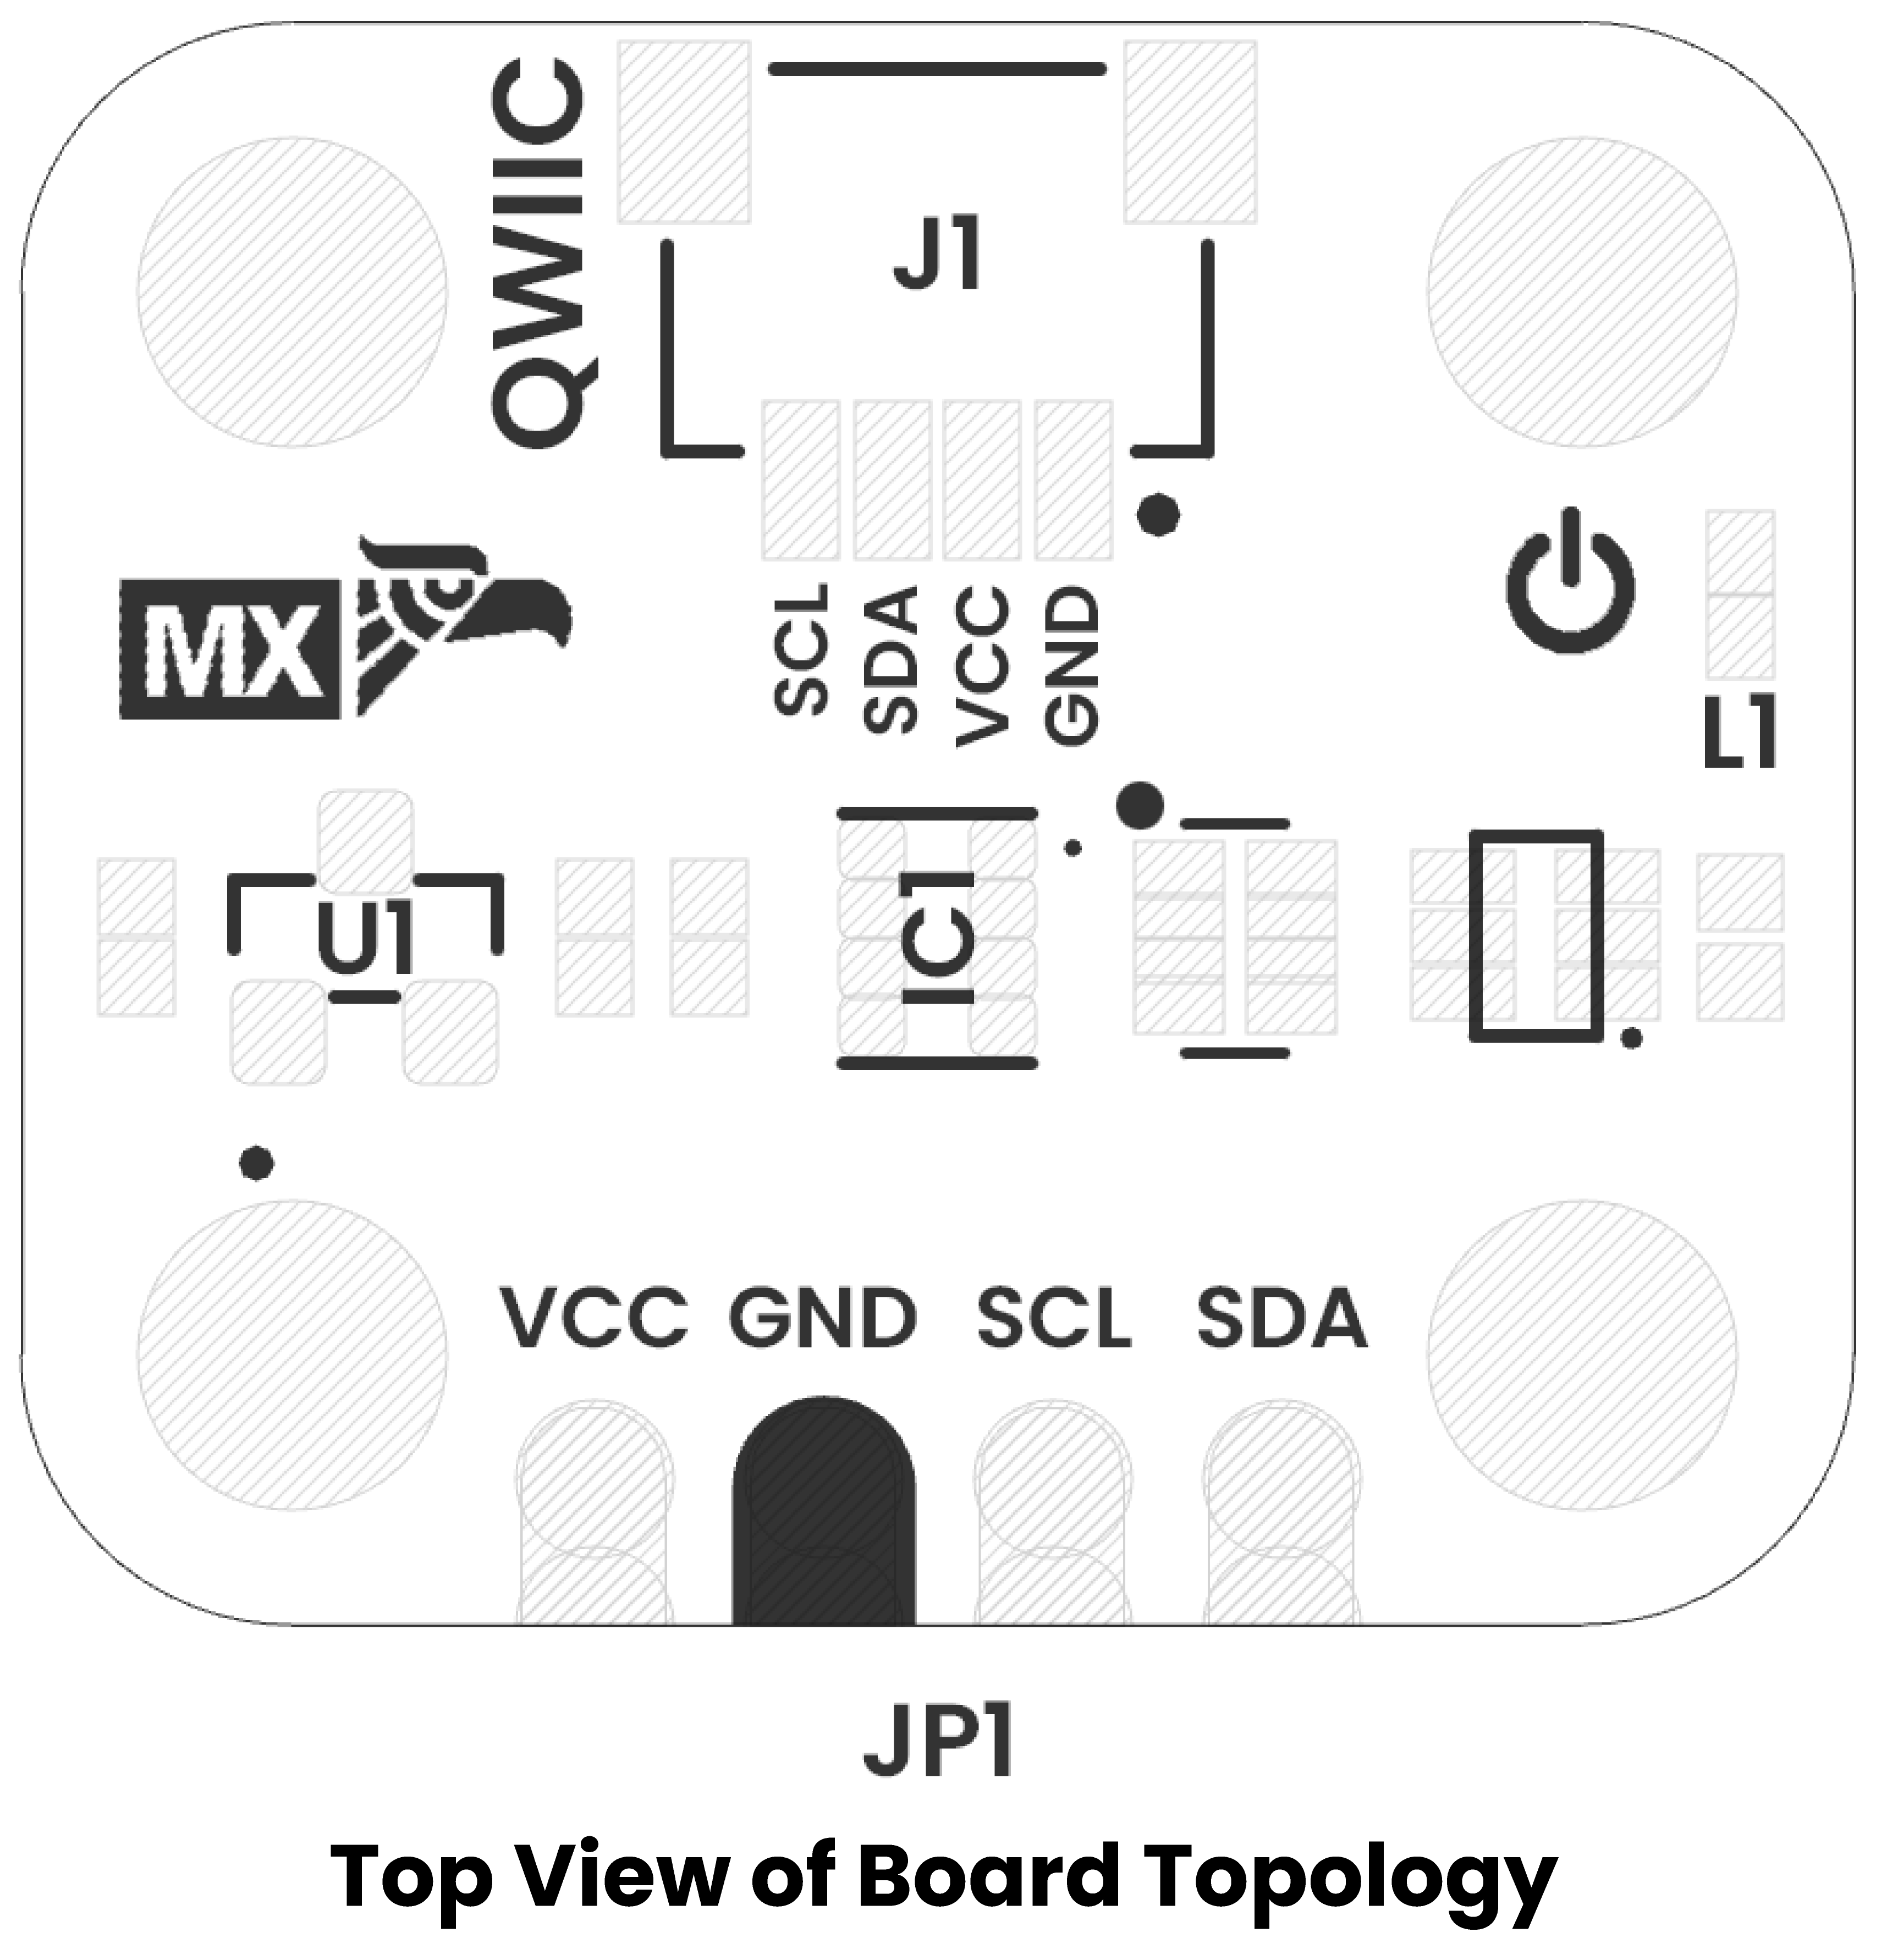
\includegraphics[width=0.7\textwidth]{en_unit_topology_v_1_0_0_icp10111_barometric_pressure_sensor.png}
\caption{System Topology}
\label{fig:en-unit-topology-v-1-0-0-icp10111-barometric-pressure-sensor-png}
\end{figure}



\subsubsection{Processor & Memory}


\begin{table}[H]
\centering
\small
\begin{tabular}{|l|l|l|l|}
\hline
Parameter & Value & Unit & Notes \\
\hline
CPU & Dual-core Xtensa LX6 & 240 MHz & 32-bit RISC \\
Flash Memory & 4 MB & MB & External SPI Flash \\
SRAM & 520 KB & KB & Internal SRAM \\
RTC Memory & 16 KB & KB & Ultra Low Power \\
\hline
\end{tabular}
\caption{Especificaciones técnicas}
\end{table}


\subsubsection{Power Specifications}


\begin{table}[H]
\centering
\small
\begin{tabular}{|l|l|l|l|l|l|}
\hline
Parameter & Min & Typ & Max & Unit & Conditions \\
\hline
Supply Voltage & 2.2 & 3.3 & 3.6 & V & Normal Operation \\
Active Current & - & 160 & 260 & mA & Wi-Fi Tx @ 19.5dBm \\
Sleep Current & - & 5 & 10 & µA & Deep Sleep Mode \\
Standby Current & - & 240 & 350 & µA & Light Sleep Mode \\
\hline
\end{tabular}
\caption{Especificaciones técnicas}
\end{table}


\subsubsection{Wireless Capabilities}

\paragraph{Wi-Fi Specifications}
\begin{itemize}
\item \textbf{Standards}: 802.11 b/g/n (2.4 GHz)
\item \textbf{Data Rate}: Up to 150 Mbps
\item \textbf{Output Power}: +19.5 dBm max
\item \textbf{Antenna}: Integrated PCB antenna
\end{itemize}

\paragraph{Bluetooth Specifications}
\begin{itemize}
\item \textbf{Version}: Bluetooth v4.2 BR/EDR and BLE
\item \textbf{Output Power}: +9 dBm max
\item \textbf{Range}: Up to 100m (open field)
\end{itemize}

\subsection{GPIO Configuration}


\begin{figure}[H]
\centering
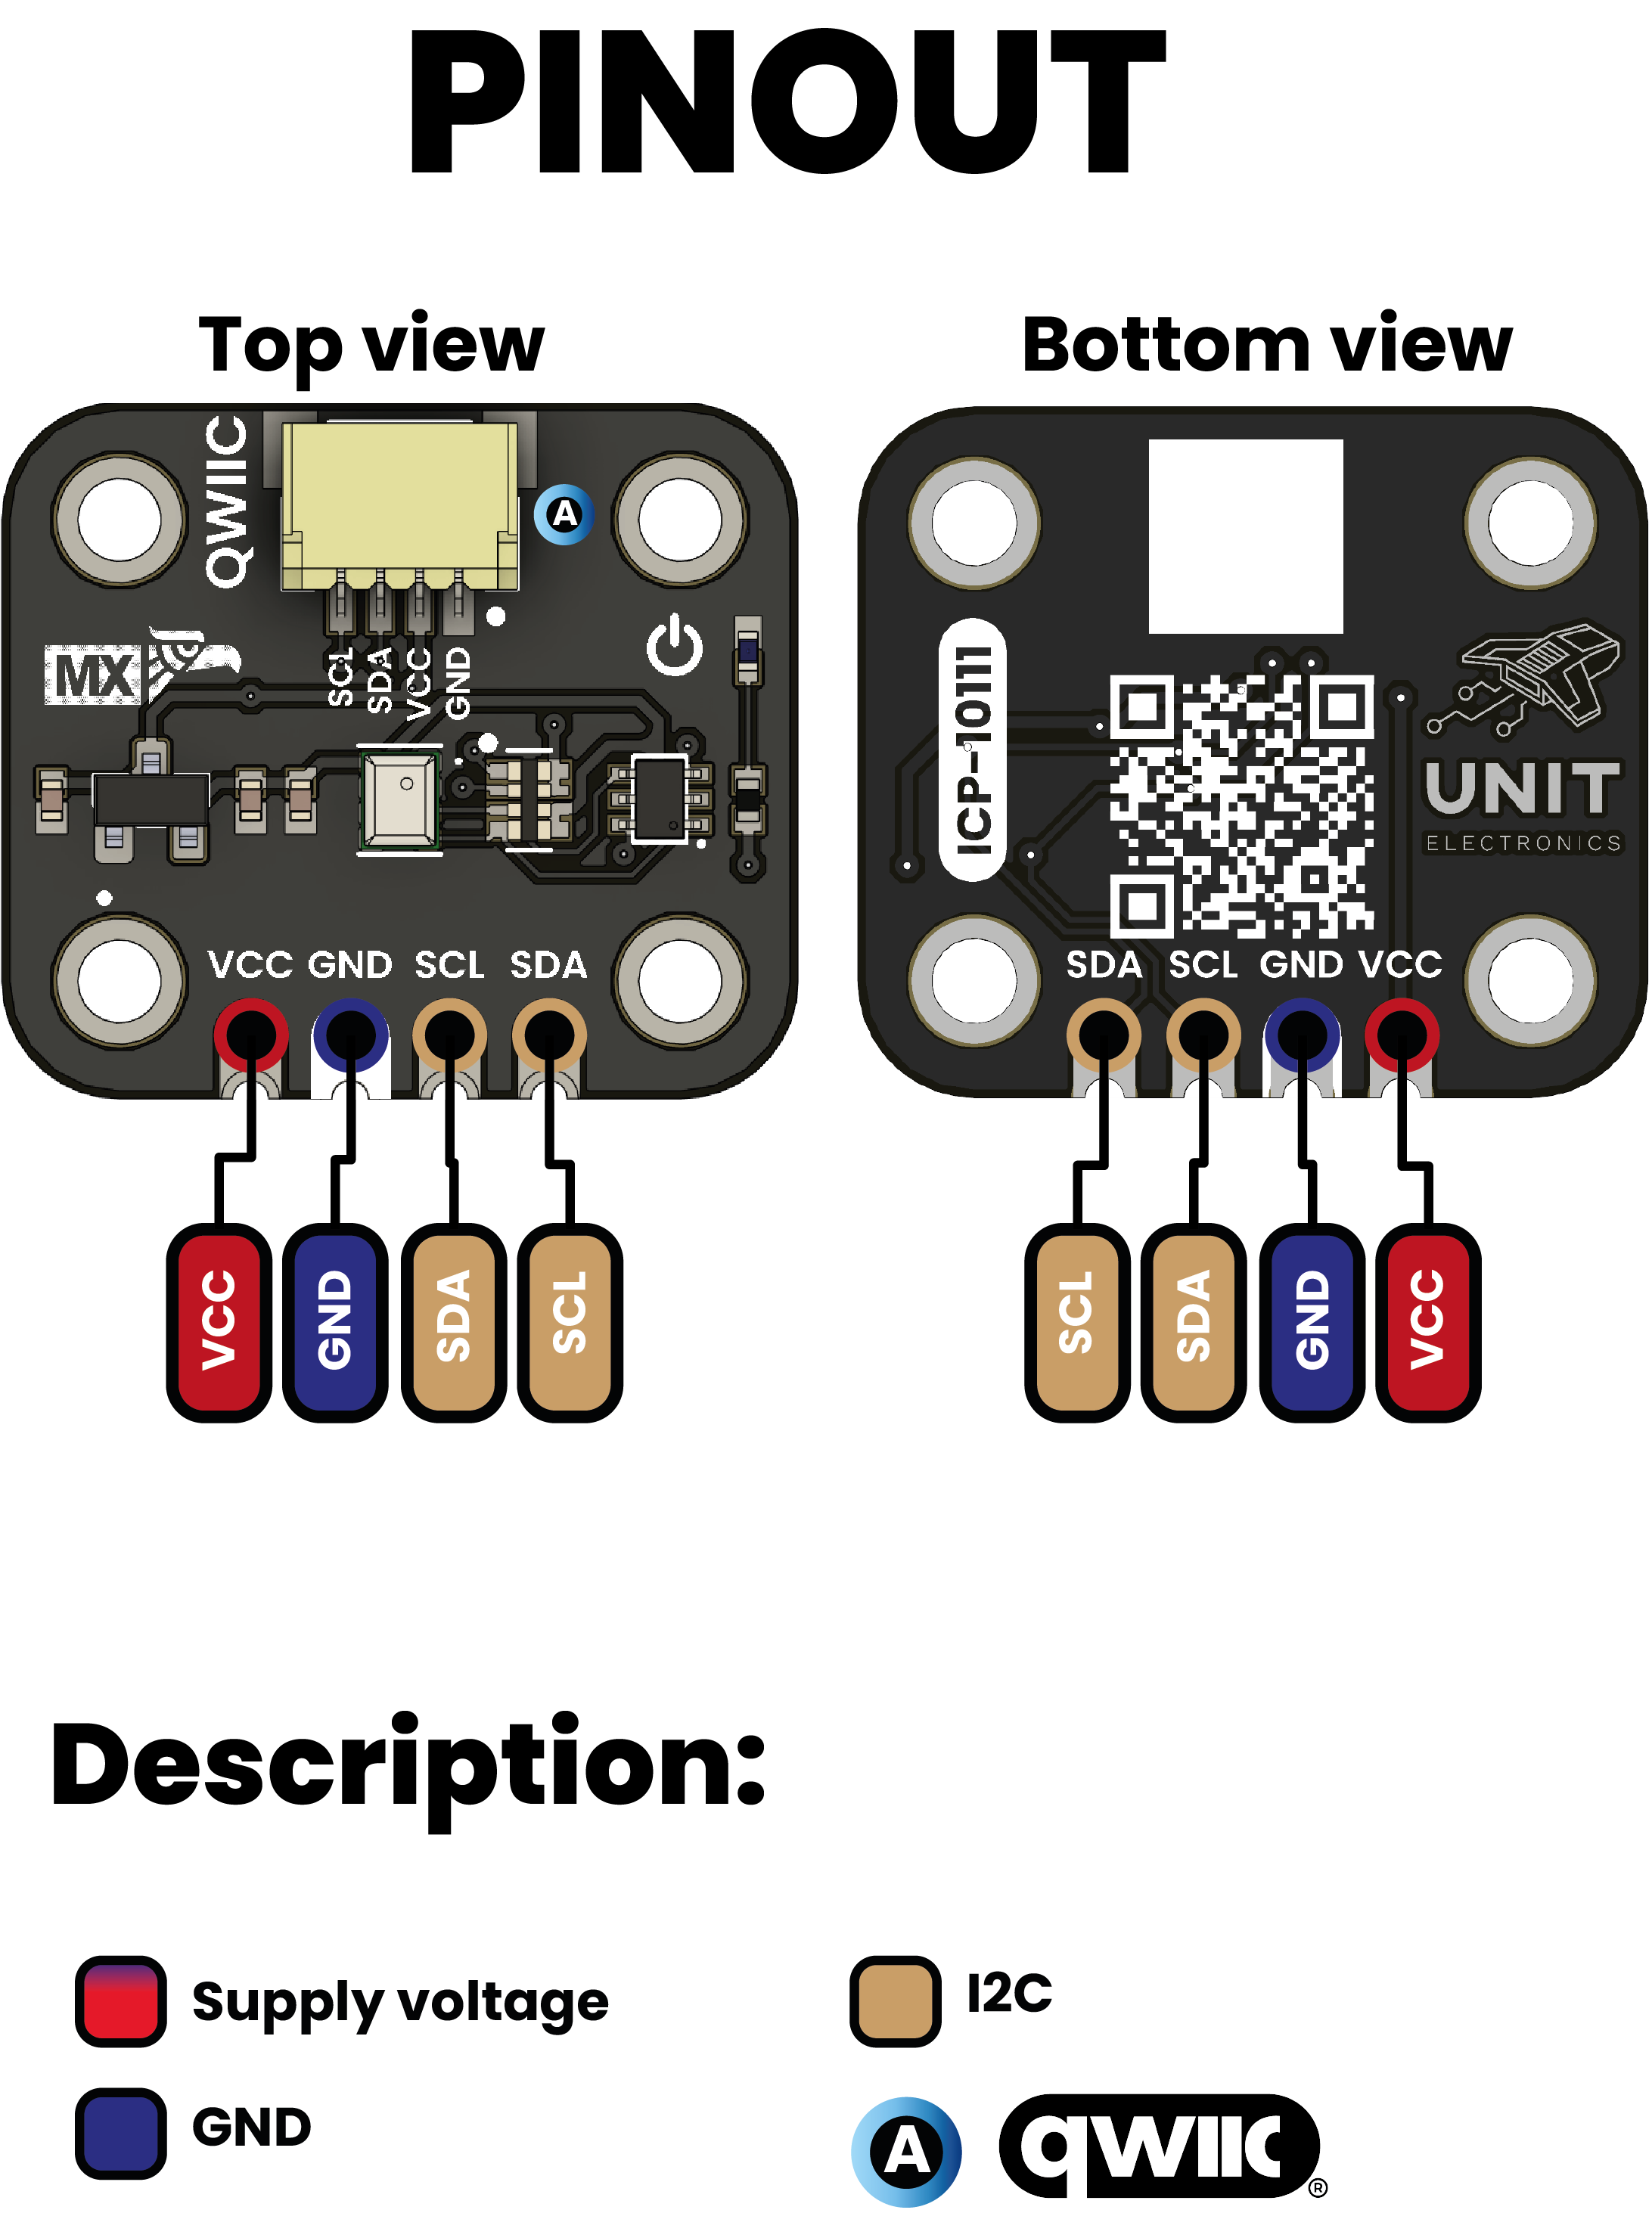
\includegraphics[width=0.9\textwidth]{en_unit_pinout_v_0_0_1_ue0094_icp10111_barometric_pressure_sensor_en.png}
\caption{Pinout Diagram}
\label{fig:en-unit-pinout-v-0-0-1-ue0094-icp10111-barometric-pressure-sensor-en-png}
\end{figure}



\subsubsection{Available Pins}


\begin{table}[H]
\centering
\small
\begin{tabular}{|l|l|l|l|l|}
\hline
Pin & Function & Voltage & Drive Current & Special Features \\
\hline
GPIO0 & Digital I/O & 3.3V & 40 mA & Boot control \\
GPIO1 & UART0_TXD & 3.3V & 40 mA & Default debug output \\
GPIO2 & Digital I/O & 3.3V & 40 mA & LED control \\
GPIO3 & UART0_RXD & 3.3V & - & Default debug input \\
GPIO4-5 & Digital I/O & 3.3V & 40 mA & General purpose \\
\hline
\end{tabular}
\caption{Especificaciones técnicas}
\end{table}


\subsubsection{ADC Capabilities}

The module includes a 12-bit SAR ADC with the following characteristics:

\begin{itemize}
\item \textbf{Resolution}: 12-bit (4096 levels)
\item \textbf{Input Range}: 0 - 3.3V
\item \textbf{Channels}: 8 channels available
\item \textbf{Sampling Rate}: Up to 2 Msps
\end{itemize}

\subsection{Communication Interfaces}

\subsubsection{UART}
\begin{itemize}
\item \textbf{Channels}: 3 hardware UART controllers
\item \textbf{Baud Rate}: Up to 5 Mbps
\item \textbf{Features}: Hardware flow control, DMA support
\end{itemize}

\subsubsection{SPI}
\begin{itemize}
\item \textbf{Channels}: 4 SPI controllers
\item \textbf{Speed}: Up to 80 MHz
\item \textbf{Modes}: Master/Slave operation
\item \textbf{Features}: DMA support, flexible pin mapping
\end{itemize}

\subsubsection{I2C}
\begin{itemize}
\item \textbf{Channels}: 2 I2C controllers
\item \textbf{Speed}: Standard (100 kHz), Fast (400 kHz), Fast+ (1 MHz)
\item \textbf{Features}: Multi-master support, 7/10-bit addressing
\end{itemize}

\subsection{Physical Characteristics}


\begin{figure}[H]
\centering
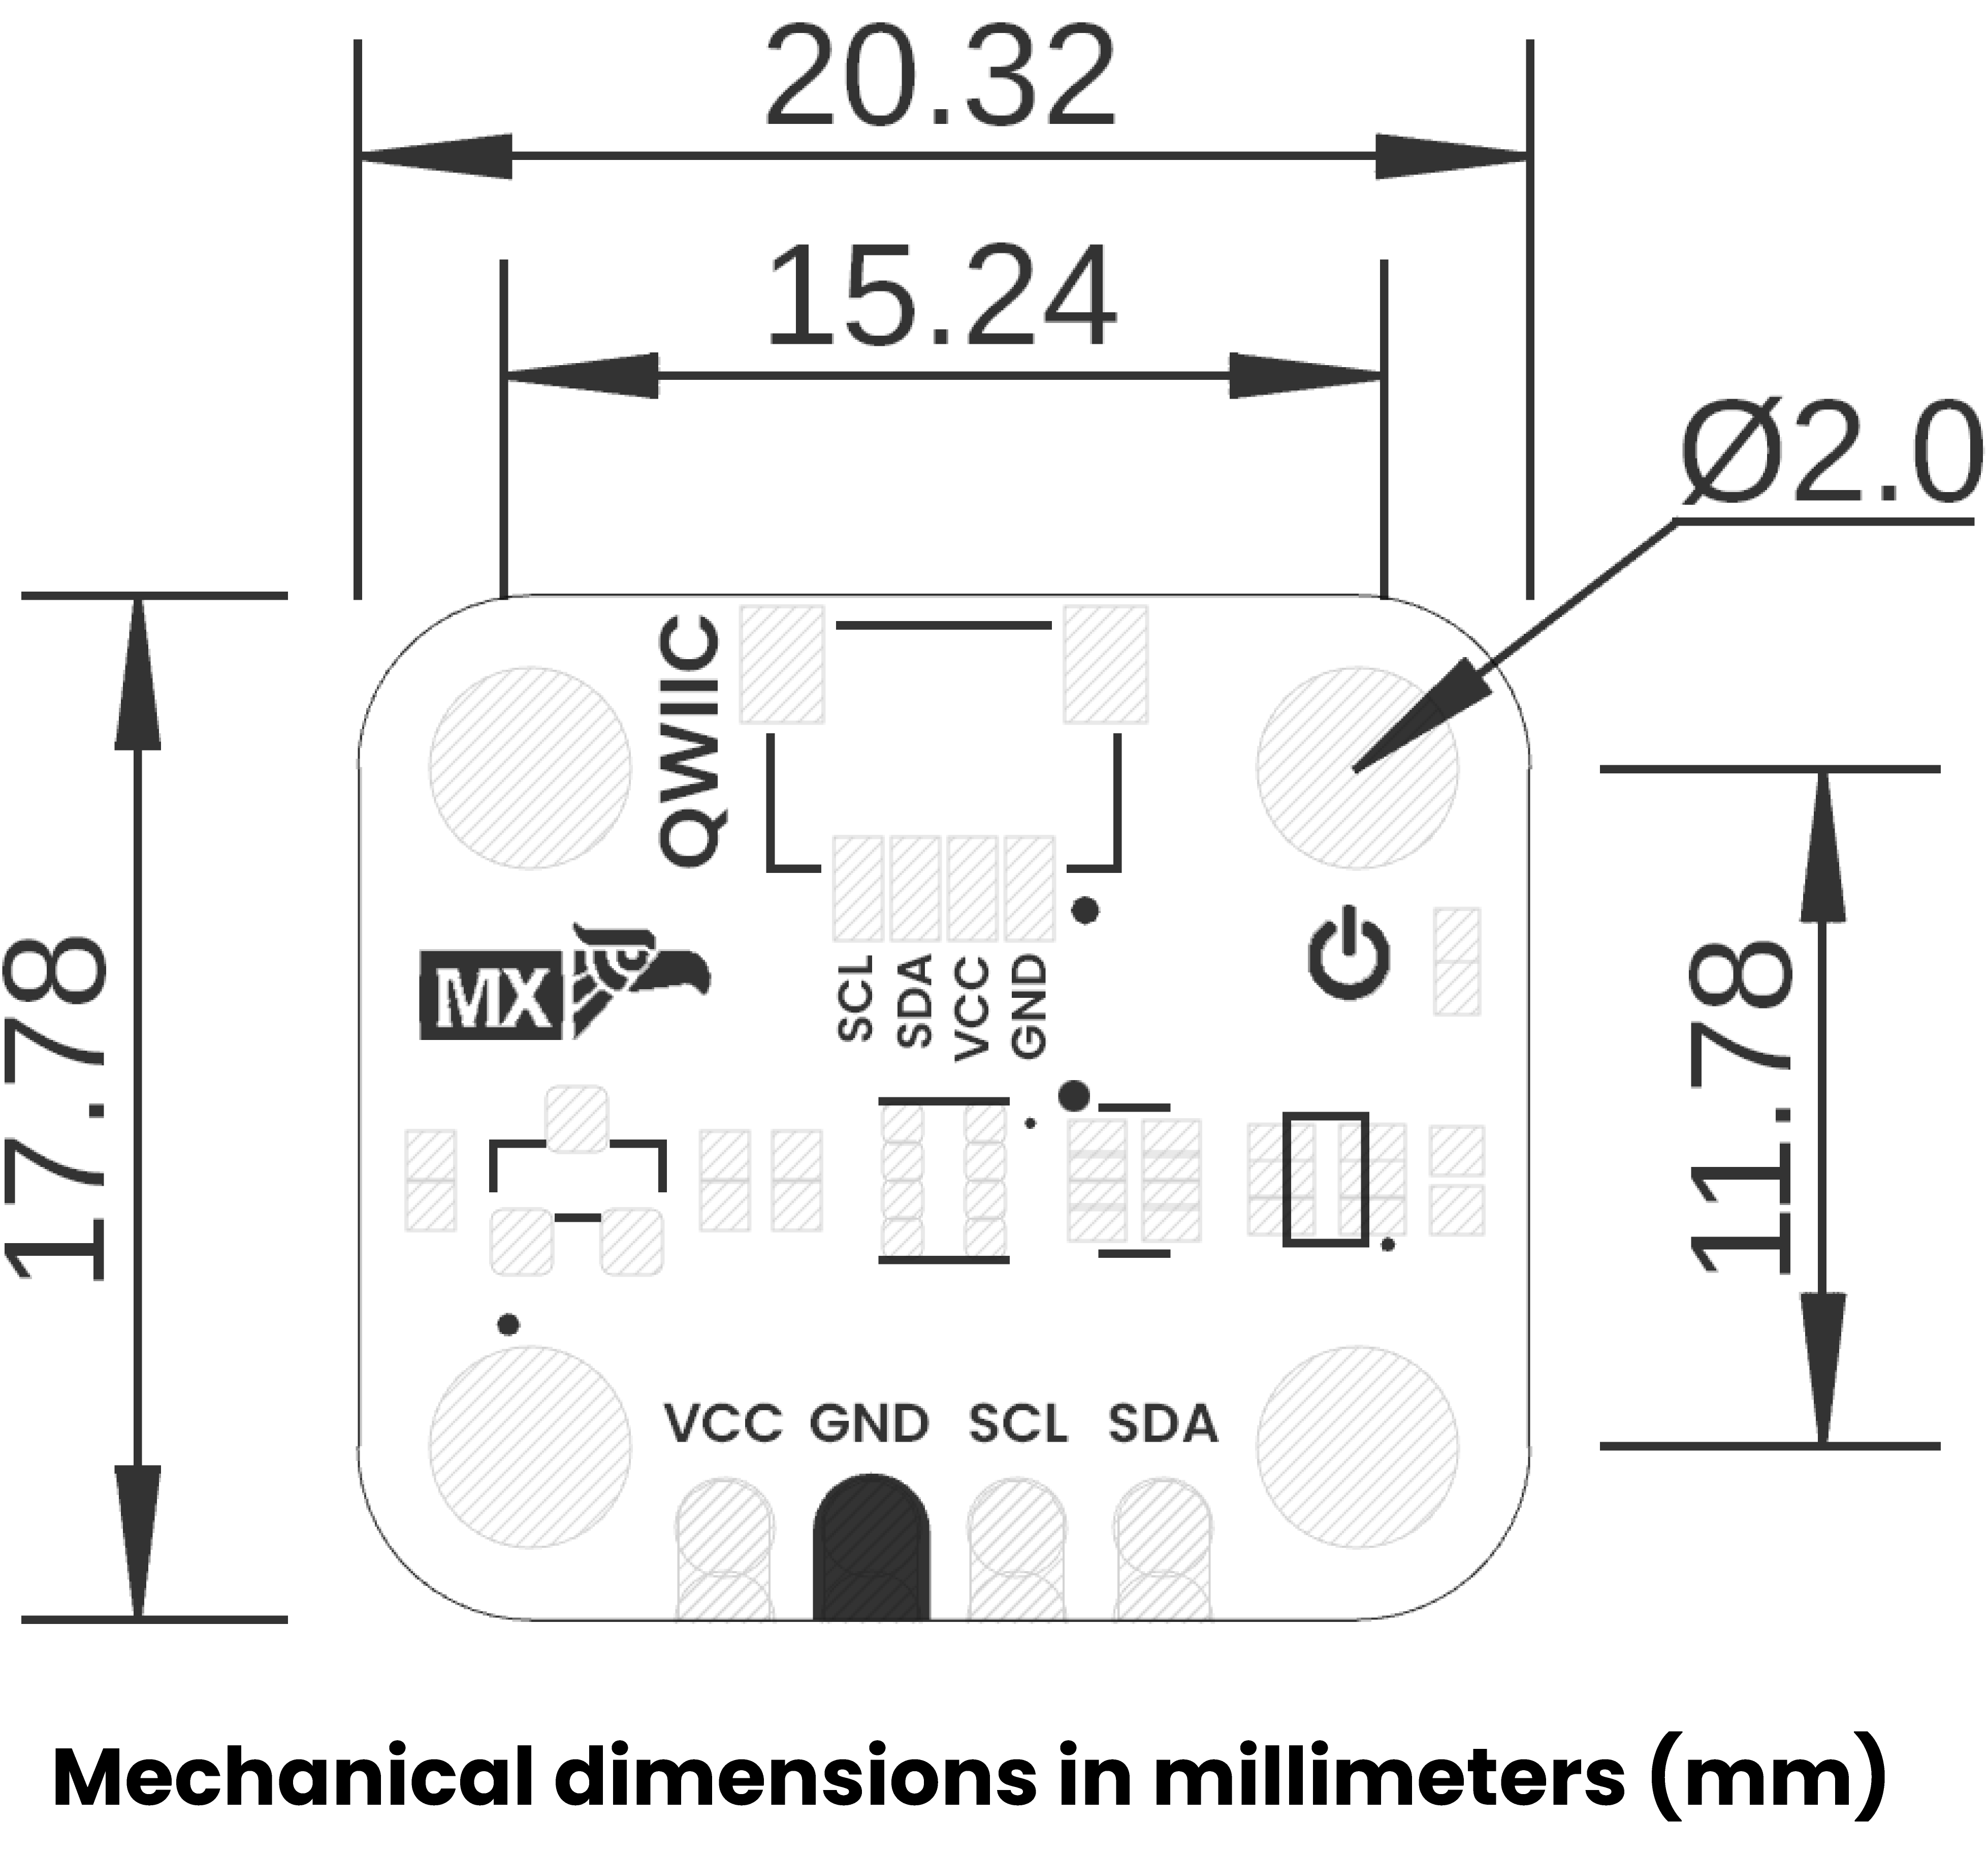
\includegraphics[width=0.6\textwidth]{en_unit_dimension_v_1_0_0_icp10111_barometric_pressure_sensor.png}
\caption{Physical Dimensions}
\label{fig:en-unit-dimension-v-1-0-0-icp10111-barometric-pressure-sensor-png}
\end{figure}




\begin{figure}[H]
\centering
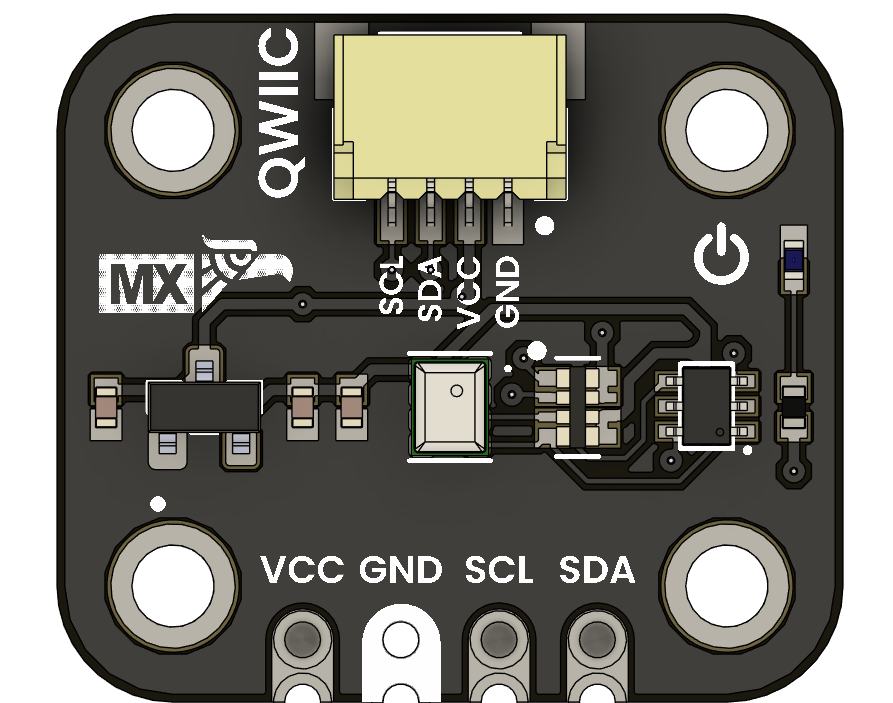
\includegraphics[width=0.7\textwidth]{en_unit_top_v_1_0_0_icp10111_barometric_pressure_sensor.png}
\caption{Top View}
\label{fig:en-unit-top-v-1-0-0-icp10111-barometric-pressure-sensor-png}
\end{figure}




\begin{figure}[H]
\centering
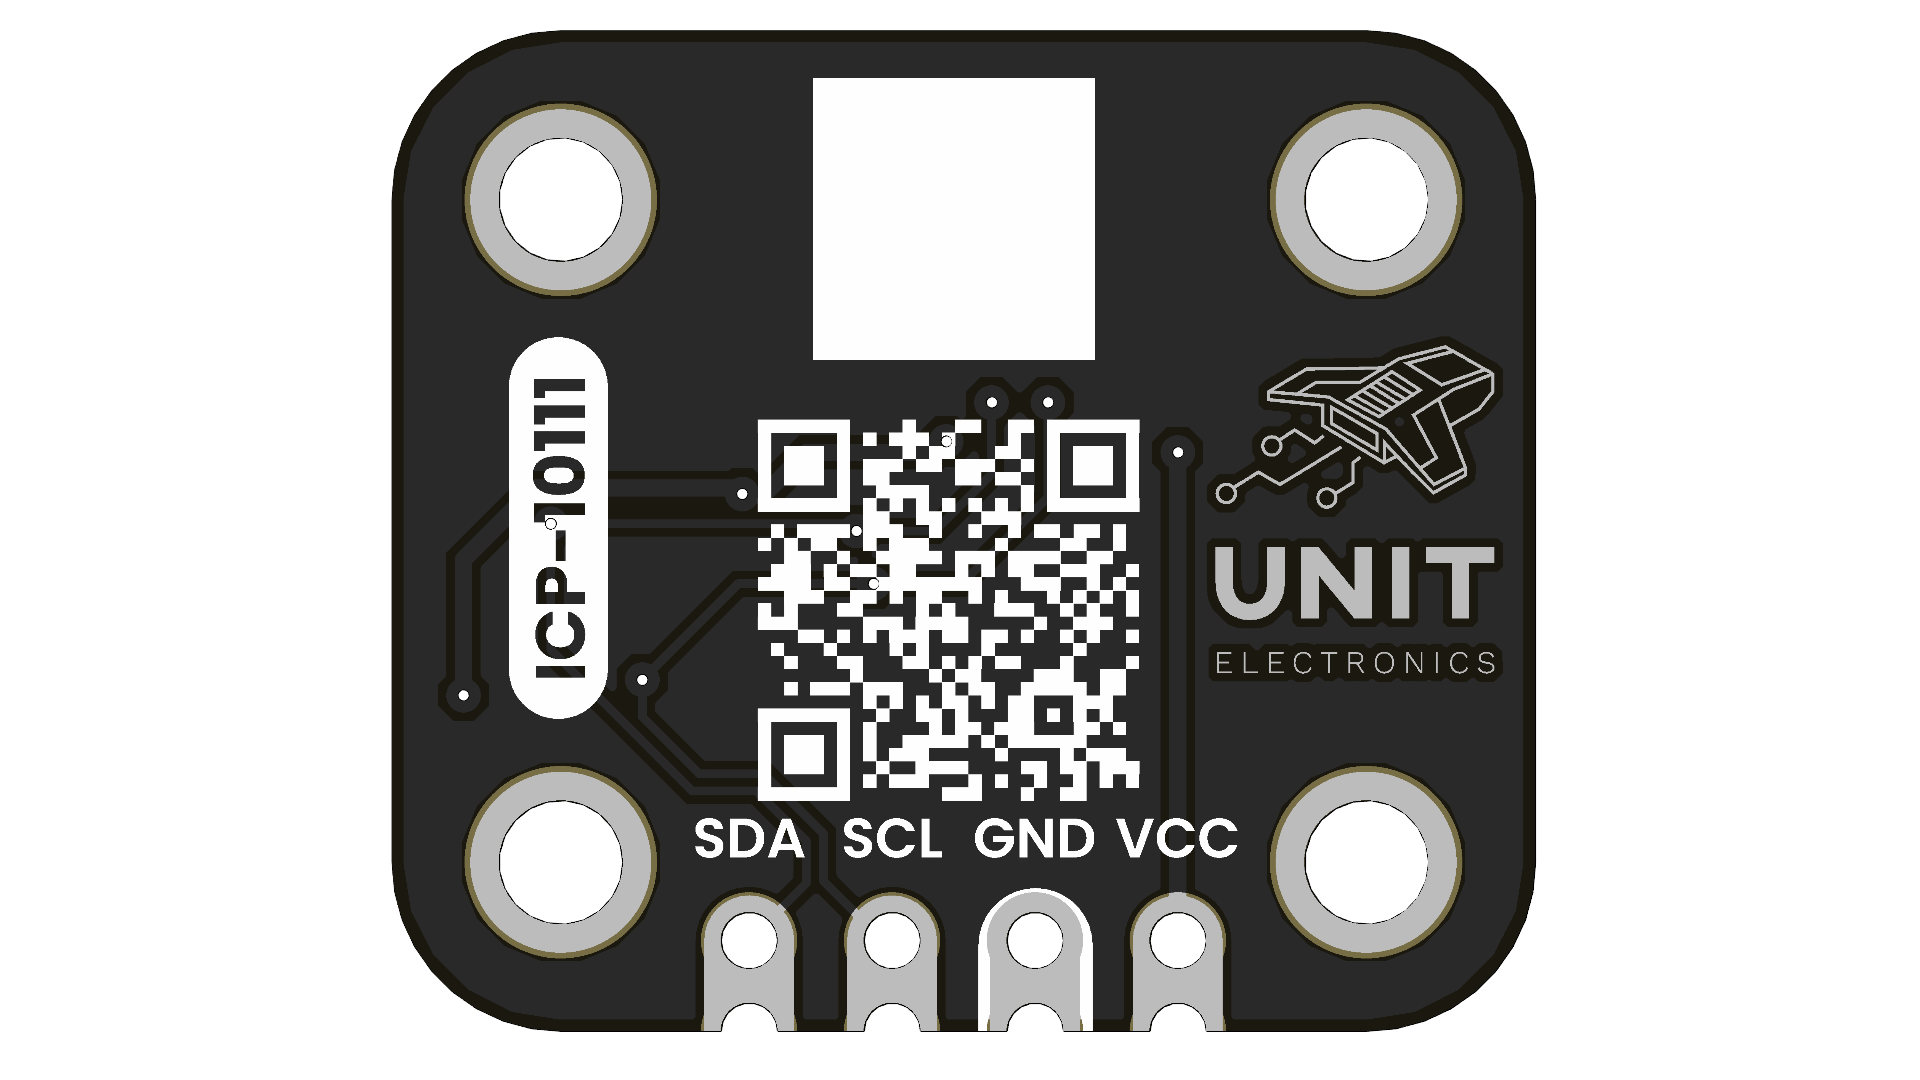
\includegraphics[width=0.7\textwidth]{en_unit_btm_v_1_0_0_icp10111_barometric_pressure_sensor.png}
\caption{Bottom View}
\label{fig:en-unit-btm-v-1-0-0-icp10111-barometric-pressure-sensor-png}
\end{figure}



\subsubsection{Package Information}


\begin{table}[H]
\centering
\small
\begin{tabular}{|c|c|c|}
\hline
Parameter & Value & Unit \\
\hline
Package Type & QFN-48 & - \\
Dimensions & 6 x 6 x 0.9 & mm \\
Pin Pitch & 0.4 & mm \\
Weight & 0.5 & g \\
\hline
\end{tabular}
\caption{Especificaciones técnicas}
\end{table}


\subsubsection{Environmental Specifications}


\begin{table}[H]
\centering
\small
\begin{tabular}{|l|l|l|l|l|}
\hline
Parameter & Min & Max & Unit & Conditions \\
\hline
Operating Temperature & -40 & +85 & °C & Commercial grade \\
Storage Temperature & -55 & +125 & °C & - \\
Humidity & 10 & 95 & %RH & Non-condensing \\
\hline
\end{tabular}
\caption{Especificaciones técnicas}
\end{table}


\subsection{Software Support}

\subsubsection{Development Environment}
\begin{itemize}
\item \textbf{Arduino IDE}: Full support with ESP32 core
\item \textbf{ESP-IDF}: Native Espressif framework
\item \textbf{PlatformIO}: Cross-platform IDE support
\item \textbf{MicroPython}: Python support for rapid development
\end{itemize}

\subsubsection{Key Libraries}
\begin{itemize}
\item WiFi & Bluetooth connectivity
\item FreeRTOS real-time operating system
\item Hardware abstraction layer (HAL)
\item Over-the-air (OTA) update support
\end{itemize}

\subsection{Applications}

The DevLab module is ideal for:

\begin{enumerate}
\item \textbf{IoT Sensors & Actuators}
\end{enumerate}
\begin{itemize}
\item Environmental monitoring
\item Smart home devices
\item Industrial automation
\end{itemize}

\begin{enumerate}
\item \textbf{Prototyping & Development}
\end{enumerate}
\begin{itemize}
\item Rapid proof-of-concept
\item Educational projects
\item Research applications
\end{itemize}

\begin{enumerate}
\item \textbf{Commercial Products}
\end{enumerate}
\begin{itemize}
\item Smart appliances
\item Wearable devices
\item Connected lighting
\end{itemize}

\subsection{Safety & Compliance}

\subsubsection{Certifications}
\begin{itemize}
\item \textbf{FCC}: Part 15.247 (USA)
\item \textbf{CE}: EN 300 328, EN 301 489 (Europe)
\item \textbf{IC}: RSS-210 (Canada)
\end{itemize}

\subsubsection{Safety Features}
\begin{itemize}
\item \textbf{ESD Protection}: ±2kV HBM on all pins
\item \textbf{Latch-up Immunity}: ±100mA
\item \textbf{Thermal Protection}: Automatic thermal shutdown
\end{itemize}

\subsection{Ordering Information}


\begin{table}[H]
\centering
\small
\begin{tabular}{|l|l|l|l|}
\hline
Part Number & Description & Package & MOQ \\
\hline
DEVLAB-001 & Standard Module & Tray & 100 \\
DEVLAB-001R & RoHS Compliant & Tape & Reel & 1000 \\
DEVLAB-DEV & Development Kit & Individual Box & 1 \\
\hline
\end{tabular}
\caption{Especificaciones técnicas}
\end{table}


\subsection{Revision History}


\begin{table}[H]
\centering
\small
\begin{tabular}{|c|c|c|}
\hline
Version & Date & Changes \\
\hline
1.0 & 2025-07-18 & Initial release \\
\hline
\end{tabular}
\caption{Especificaciones técnicas}
\end{table}


\subsection{Schematics}


\begin{figure}[H]
\centering
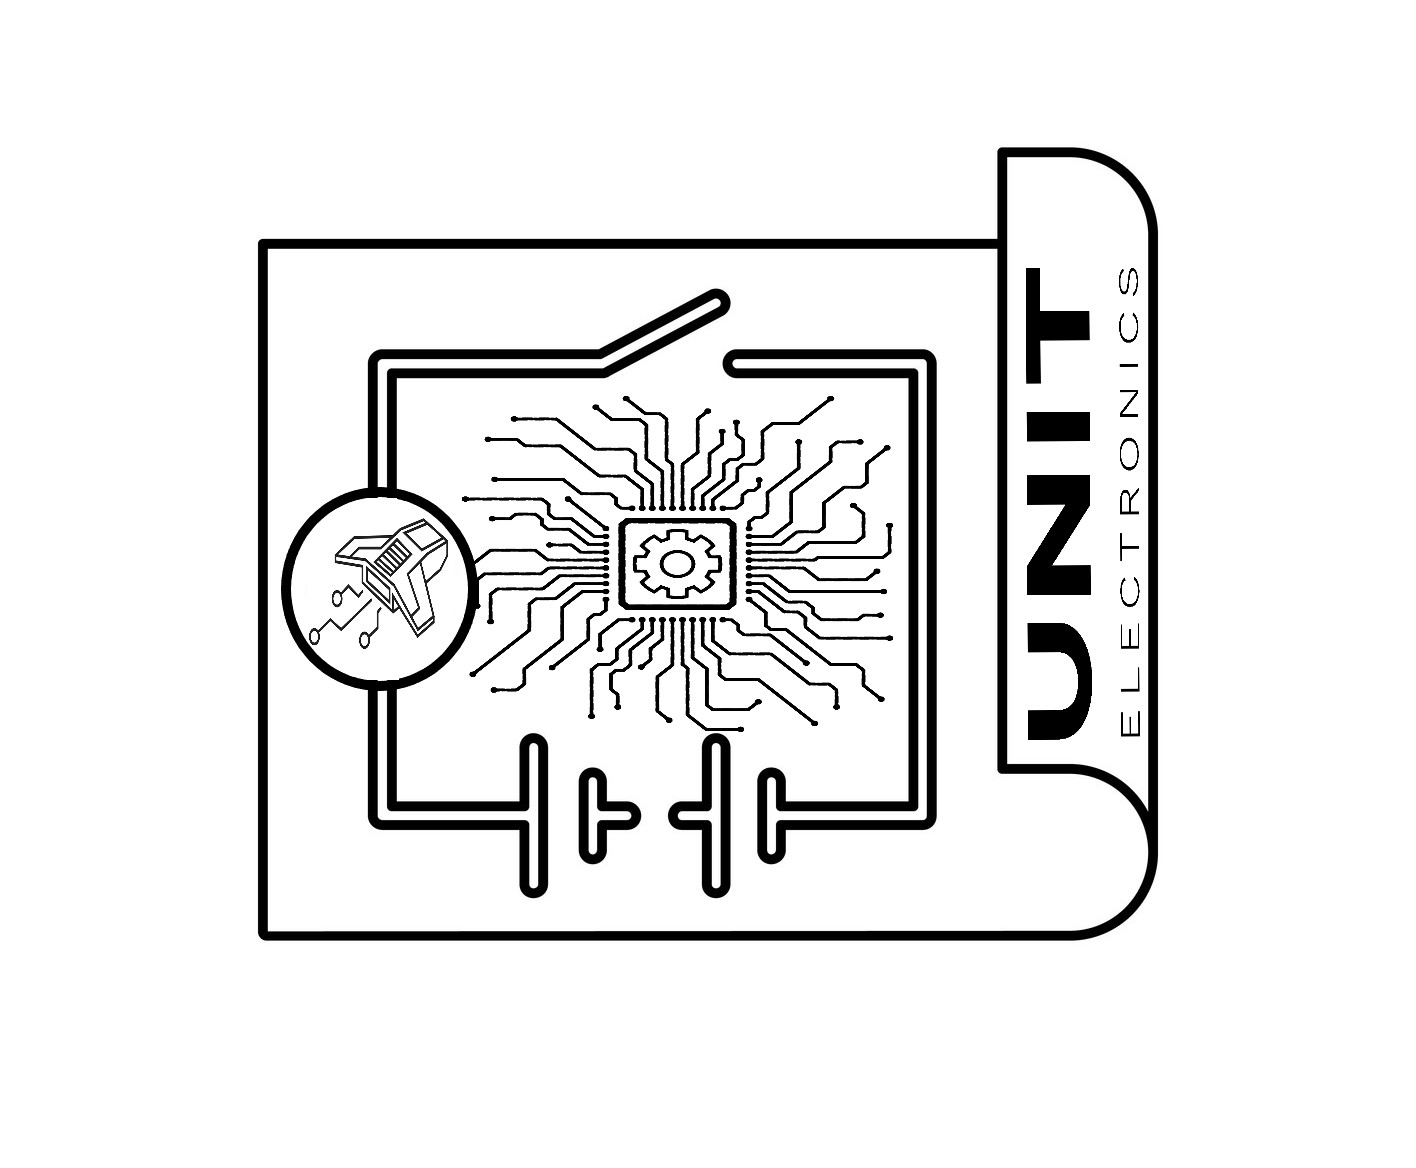
\includegraphics[width=\textwidth]{en_Schematics_icon.jpg}
\caption{Circuit Schematic}
\label{fig:en-Schematics-icon-jpg}
\end{figure}



---

\textit{For technical support and additional information, visit our website or contact our engineering team.}


\end{document}
